%%%%%%%%%%%%%%%%%%%%%%%%%%%%%%%%%%%%%%%%%%%%%%%%%%%%%%%%%%%
%% I18n

\section{Internacionalización}\label{i18n:internacionalizacion}

\subsection{Qué entendemos por internacionalización (i18n)}\label{i18n:que-entendemos-i18n}

El principal sentido de la i18n es diseñar el código de tal forma que el programa sea fácil de localizar y distribuir internacionalmente. Para ello es importante considerar los siguientes aspectos:

\begin{enumerate}
	\item \textbf{Diseño y desarrollo que facilite la localización o la distribución internacional:}
	Por ejemplo, usar el sistema Unicode para la codificación de caracteres, usar tipografías compatibles, controlar la concatenación de cadenas y evitar que el código dependa de strings pertenecientes a la \lsc{UI}.
	
	\item \textbf{Crear métodos específicos para la localización:}
	Añadir etiquetas para habilitar texto bidireccional, la identificación de idiomas (\href{https://es.wikipedia.org/wiki/ISO_639}{ISO-639}) o hacer la \lsc{UI} compatible con el texto vertical y otras tipografías ajenas al alfabeto latino.
	
	\item \textbf{Preparar el código para que se ajuste a las preferencias locales, lingüísticas o culturales:}
	Esto supone incorporar características y datos de localización predefinidos a partir de bibliotecas existentes o de preferencias de usuario, formatos de fecha y hora, calendarios locales, formatos y sistemas de números, ordenamiento y presentación de listas, uso de nombres personales y formas de tratamiento, etc.
	
	\item \textbf{Separar del código los elementos localizables:}
	De este modo podrán cargarse o seleccionarse alternativas localizadas según lo que determinen las preferencias internacionales del usuario.
\end{enumerate}

\subsection{Qué entendemos por localización (l10n)}\label{i18n:que-entendemos-l10n}
Se entiende por l10n la adaptación del software con el objetivo de adecuarlo a las necesidades lingüísticas, culturales o incluso legales de un mercado, país o localidad en concreto.

Más allá de considerar la traducción de la documentación y la interfaz de usuario, la l10n es bastante más compleja pues además implica ajustar:
\begin{itemize}
	\item Formatos numéricos, de fecha y de hora.
	\item Uso de símbolos de moneda.
	\item Uso del teclado.
	\item Algoritmos de comparación y ordenamiento.
	\item Símbolos, íconos y colores.
	\item Texto y gráficos que contengan referencias a objetos, acciones o ideas que en una cultura dada puedan ser objeto de mala interpretación u ofensas.
	\item Diferentes exigencias legales.
\end{itemize}

\subsection{Implementación}\label{i18n:implementacion}
Tal como se ha mencionado en el apartado \nameref{principios:vision-general-desarrollo}), muchos aspectos del diseño se irán definiendo en la medida que se obtenga más información de los desafíos y los requerimientos del software.

Dada la enorme cantidad de texto que se espera del proyecto, es de vital importancia considerar desde el principio los desafíos de la i18n y l10n.
Al mismo tiempo, dado el desconocimiento de nuestra propia implementación, no podremos restringir \textit{a priori} la elección de un mecanismo a otro. Por lo tanto el enfoque debe tener las siguientes consideraciones:

\subsubsection{Exploración}\label{i18n:exploracion}
Durante el desarrollo de las distintas funciones que requieran strings y assets con texto visibles por el jugador (letreros, videos, mapas), será importante considerar algún sistema para el manejo de los texto por cada idioma que soportará el juego.
En este sentido, al mismo tiempo que los strings sean almacenados de forma eficiente para el uso en la ejecución del programa, deberán facilitar la modificación continua de las cadenas como parte integral del desarrollo.

\subsubsection{Codificación}\label{i18n:codificacion}
Para la codificación de caracteres se usará el sistema Unicode bajo el formato UTF-8 en \emph{todos} los textos de contenido del juego.

\subsubsection{Estructura de los directorios de l10n}
En la carpeta raíz del proyecto se encontrará la carpeta locales. Dentro de ésta habrá una carpeta por cada idioma según su código ISO-639. Dentro, se crearán las mismas subcarpetas y archivos manteniendo la misma estructura de directorios. La cuenta, o cantidad de archivos y subdirectorios debe ser la misma para todos los idiomas. El idioma base para el contenido del juego será el español; no obstante los nombres de los archivos y las carpetas se deben escribir en inglés siguiendo la nomenclatura propuesta en el apartado \nameref{organizacion:nombres-de-archivos}.

\subsubsection{Diagrama del árbol de directorios}\label{i18n:arbol-de-directorios}

\begin{figure}[H]
	\centering
	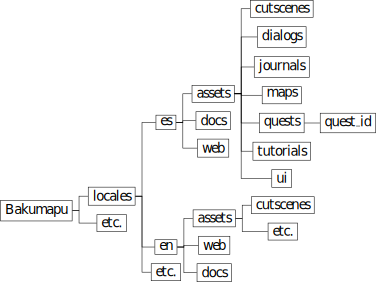
\includegraphics[]{imágenes/arbol_i18n}
	\caption{Organización de archivos de i18n.}
	\label{fig:arbolinternacionalizacion}
\end{figure}

\subsubsection{Kit de desarrollo y API}\label{i18n:toolkit-y-api}
Se estudiará la creación de un kit de herramientas para el desarrollo, específico de la l10n que interactúe con el programa y entre otras funciones permita:
\begin{itemize}
	\item Generar documentos de referencia de personajes, locaciones, quests, etc.
	\item Generar reportes de actualización en el diseño o la l10n.
	\item Comprobar límites de strings, codificación y otras especificaciones.
	\item Comprobar nombres de archivos.
	\item Control de los elementos localizados pendientes.
	\item Categorización de cambios (relevantes, irrelevantes) y prioridades.
\end{itemize}
Referencias: \href{https://drive.google.com/file/d/1OJxibGWbvxJq3_8WwmR93yzCCCvq7iu-/view?usp=sharing}{El caso de BioWare}.

\subsubsection{Godot}\label{i18n:i18n-godot}
Godot (versión 3.3) tiene implementadas dos formas de localización: a través de archivos \lsc{CSV} y mediante el uso de \textbf{gettext} (reducido).

Según este análisis previo a la implementación, el primer método es insuficiente y puede generar problemas al considerar la enorme cantidad de strings que debería contener el archivo \lsc{CSV} por cada idioma. Al ser un único archivo propone varias complicaciones al desarrollo tales como: el control de versiones, el trabajo en paralelo, algoritmos de parsing, corrupción y otros problemas.

Por otro lado, \textbf{gettext} parece ser una alternativa bastante acertada pues en principio permitiría cumplir todos los requisitos presentados en este apartado dependiendo la implementación del manejo de strings del código. Lo mejor de esta alternativa es que es uno de los estándares utilizados en los entornos de desarrollo de software, por lo que es una solución muy robusta y terminada. Además es importante destacar que cuenta con plataformas online tales como \href{https://www.transifex.com/}{Transifex} o \href{https://weblate.org}{Weblate} y mucho soporte y documentación en general.

El mayor punto en contra de \textbf{gettext} es una curva de aprendizaje mucho más inclinada, pero por otro lado los desafíos de la i18n y la l10n son de por sí muy complejos. El utilizar herramientas creadas específicamente con estos fines puede ahorrar mucho tiempo en el largo plazo y al mismo tiempo mejorar la calidad del contenido.

\subsubsection{Toma de decisiones}\label{i18n:decisiones-i18n}
Dado que aún no hay código implementado la decisión de usar un sistema como \textbf{gettext} o implementar una \lsc{API} propia, se puede tomar más adelante. Lo importante es que en el diseño narrativo, se utilicen templates que permitan a futuro la utilización de scripts para acondicionar los formatos una vez se tenga decidido el sistema y su implementación.

\subsubsection{Otras referencias}\label{i18n:otras-referencias}

\begin{enumerate}
\item \sloppy\href{https://daydigital.com/video-game-internationalization-best-practices}{Video Game Internationalization: Best Practices for Localization Friendly Architecture}

\item \href{https://docs.godotengine.org/en/latest/tutorials/i18n/localization_using_gettext.html}{Godot: Localization using gettext}

\item \href{https://stackoverflow.com/a/15343103/14377142}{Gettext or Database translation?}

\item \href{https://www.joelonsoftware.com/2003/10/08/the-absolute-minimum-every-software-developer-absolutely-positively-must-know-about-unicode-and-character-sets-no-excuses/}{The Absolute Minimum Every Software Developer Absolutely, Positively Must Know About Unicode and Character Sets}
\end{enumerate}